\chapter{Conclusion \& Future Plan} \label{cha summary}
% **************************** Define Graphics Path **************************
 \graphicspath{{Figs/}}
 
%\textbf{Note:}
%\begin{enumerate}
%  \item Generalized thick strip modelling for vortex-induced vibration of long
%flexible cylinders, 3D model	
%  \item Numerical studies on VIV of two cylinders in tandem were mainly conducted at rela- tively low Reynolds numbers 14-19 below
%  \item The studies of VIV of rigidly connected two cylinders in turbulent flows are rare.
%  \item biological application: flagella
%\end{enumerate}
%
%check oxford website

This chapter summaries the content of the entire report and plans the research work in the future.

\section{Conclusion}
This Ph.D.\ project reviews the dynamic characteristics of an elastically mounted cylinder in detail, and various research about multiple stationary or elastically mounted cylinders. Both experimental and numerical studies were addressed. The tendency is that more and more researches are carried out by numerical simulations rather than experiments. It can be seen that, despite applications in many fields including offshore and civil engineering, the dynamics of multiple cylinders exposed to a steady flow is still not fully understood. This research investigates the interaction between two cylinders in still water, which aims to simplify the case by excluding the influence from fluid flow. The current research implements the finite element method with arbitrary Lagrangian-Eulerian (ALE) method to solve the two-dimensional (2D) Navier-Stokes equations directly. The turbulence model was not included (i.e. it is DNS), because all current simulations had a low Reynolds number $ Re=100 $. However, to accommodate situations with higher Reynolds numbers, the future simulation may apply the SST k-omega model (i.e. a RANS model) or LES genre models. The code was used to simulate the simplified case (see \Cref{fig:twocylinders}) with five determining non-dimensional groups (see \Cref{tablecasegroups}). Simulation results demonstrated that resonance occurred at around $ f_1=0.8f_n $, and the increase of C1's amplitude $ A_1 $ raised C2's amplitude $ A_2 $ yet decreased the amplitude magnification factor ($ A_2/A_1 $). Vibration centre shift occurred at $ G=3 $ and became increasingly obvious with the increase of $ A_1 $ and $ f_1 $.

\section{Future Plan} \label{sec future work}
In terms of my future work, more simulation cases with different gap ratios and C1's amplitude will be carried out, and further study will focus on cases with $ 0.01 \leq G \leq 0.1 $. The Reynolds number will also be increased to explore cases with complicated flow regimes \cite{tatsuno1990visual}. In order to conduct simulations with high Reynolds numbers, 3 dimensional numerical model and RANS turbulence model will be employed. Various mass ratios will be tested to explore their effects on the cylinder interaction results. Compressible Navier-Stokes equations may be applied for investigation on high mass ratio conditions (e.g. $ m^*=250 $ in air). Also, another case setup with transverse cylinder motion will be further investigated. This transverse setup is currently difficult, as the mesh is so distorted that the calculation diverges during the transverse vibration. The 2DOF movement of the responding cylinder will be studied with 3D model with RANS turbulence model in high Reynolds numbers conditions for the best approximation to engineering reality. To deal with the computationally expensive 3D models, the parallel computing technique will be employed. In addition, possible options for the applied numerical model is listed in \Cref{simoptions}.
  
In terms of analysis and discussion, the force coefficient will be examined, and the detailed mechanism of the interaction will be further investigated by flow visualisation. The vortex patterns and streak lines will be compared with flow regimes classified by Tatsuno \& Bearman \cite{tatsuno1990visual}. The occurrence of resonance at $ f_1=0.8f_n $ rather than $ f_1=f_n $ will be further discussed with links to the added mass. Quantitative relationship between input parameters and the output data will be constructed.

Further researches may also investigate other computational fluid dynamics topics such as VIV energy harvesting and micro-organism flagella motion.
 
A research timetable in the form of Gantt chart is presented in the next two pages. 
 
  \begin{table} [tbh]
  	\centering
  	\caption{Simulation Options}
  	\label{simoptions}
  	{\renewcommand{\arraystretch}{1.2}
  		\begin{tabular}{|c|c|c|} \hline 
  			%			Option  & 1st & 2nd  \\ \hline
  			\textbf{Dimensions} & 2D & 3D \\ \hline
  			\textbf{DOF for Cylinder 2}& 1DOF & 2DOF\\ \hline
  			\textbf{Motion of Cylinder 1} & Inline & Transverse \\ \hline 
  			\textbf{Turbulence Model} & DNS (low $ Re_m $) & RANS (high $ Re_m $) \\ \hline
  			\textbf{NS Equations} & Incompressible (water, low $ m^* $) & Compressible (air, high $ m^* $) \\ \hline
  		\end{tabular}
  	}
  \end{table}
 
% \cleardoublepage
% \clearpage



%\section{Research Time Table}

% 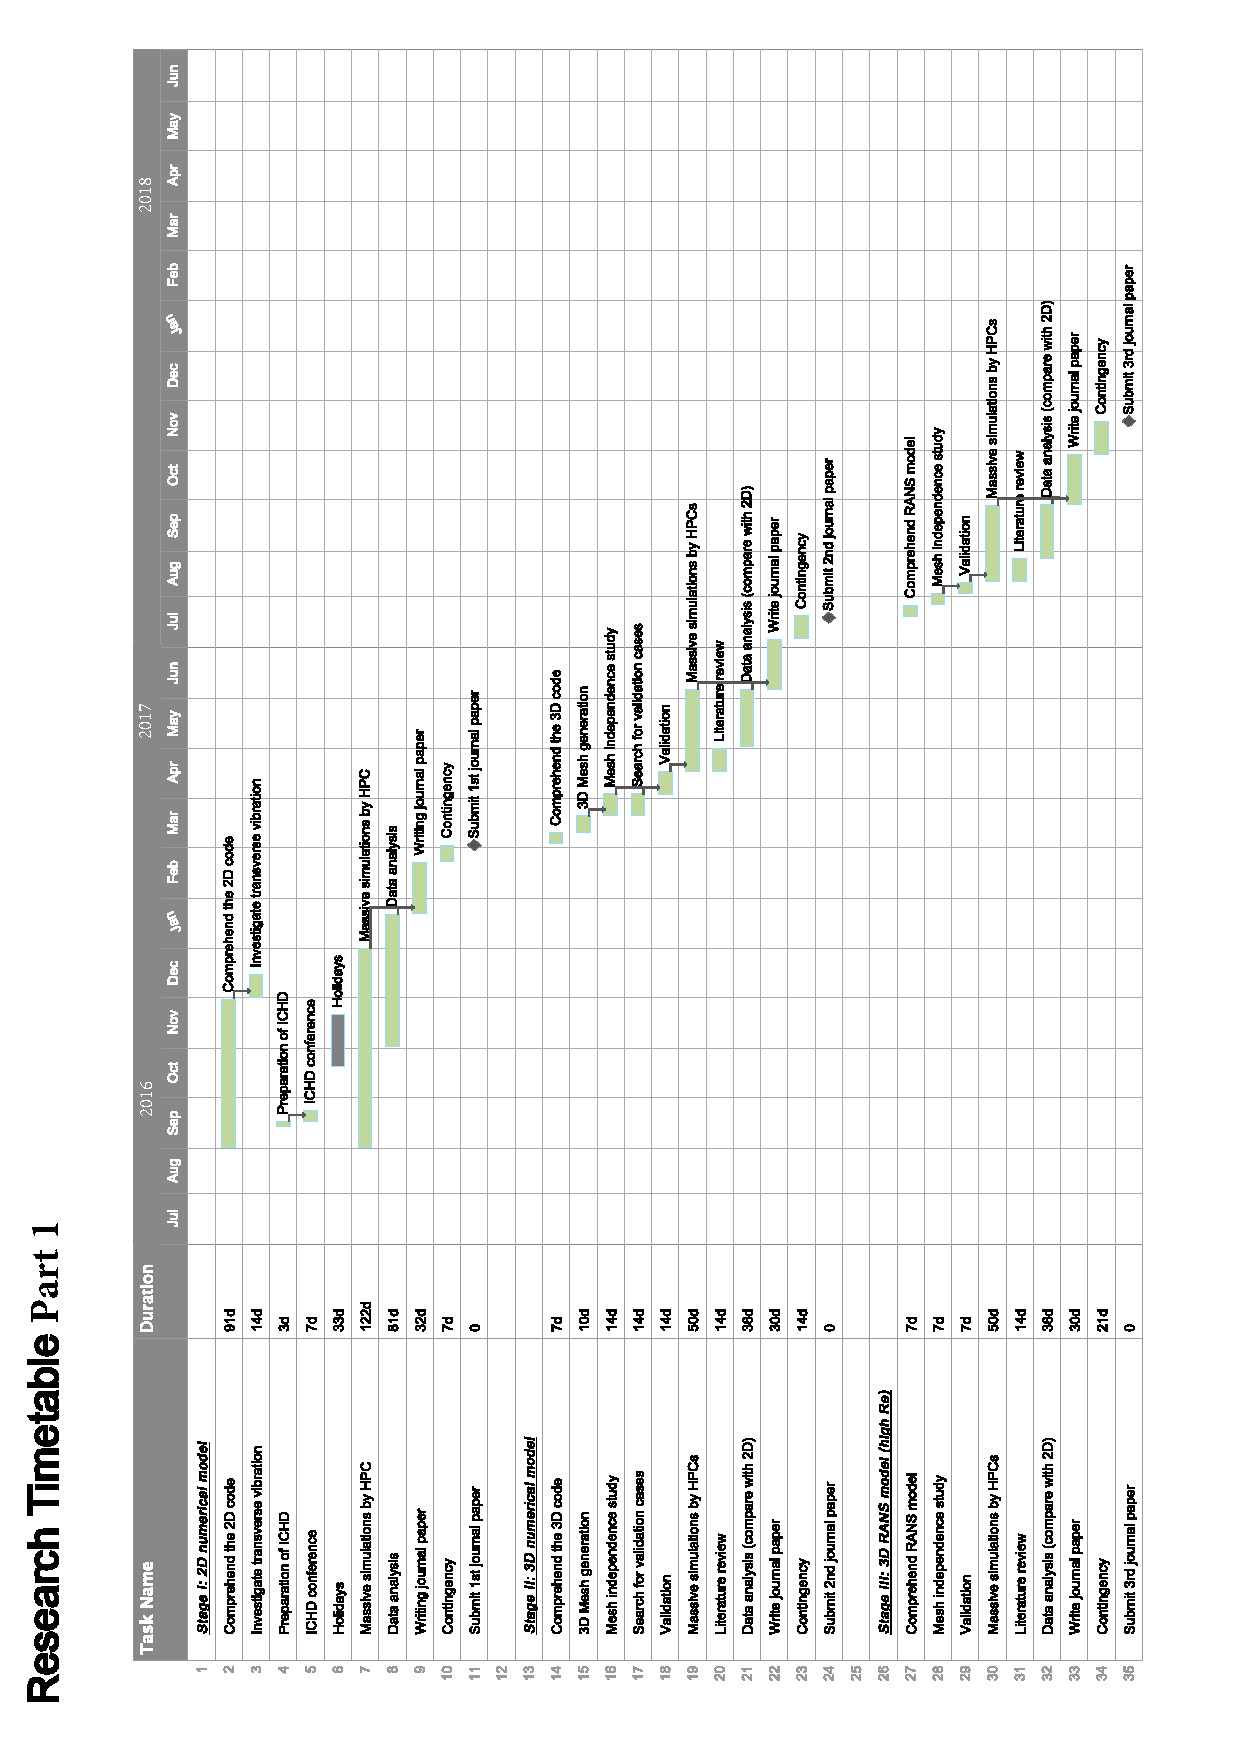
\includepdf[pages={1}]{Figs/Research Timetable (1)}
% 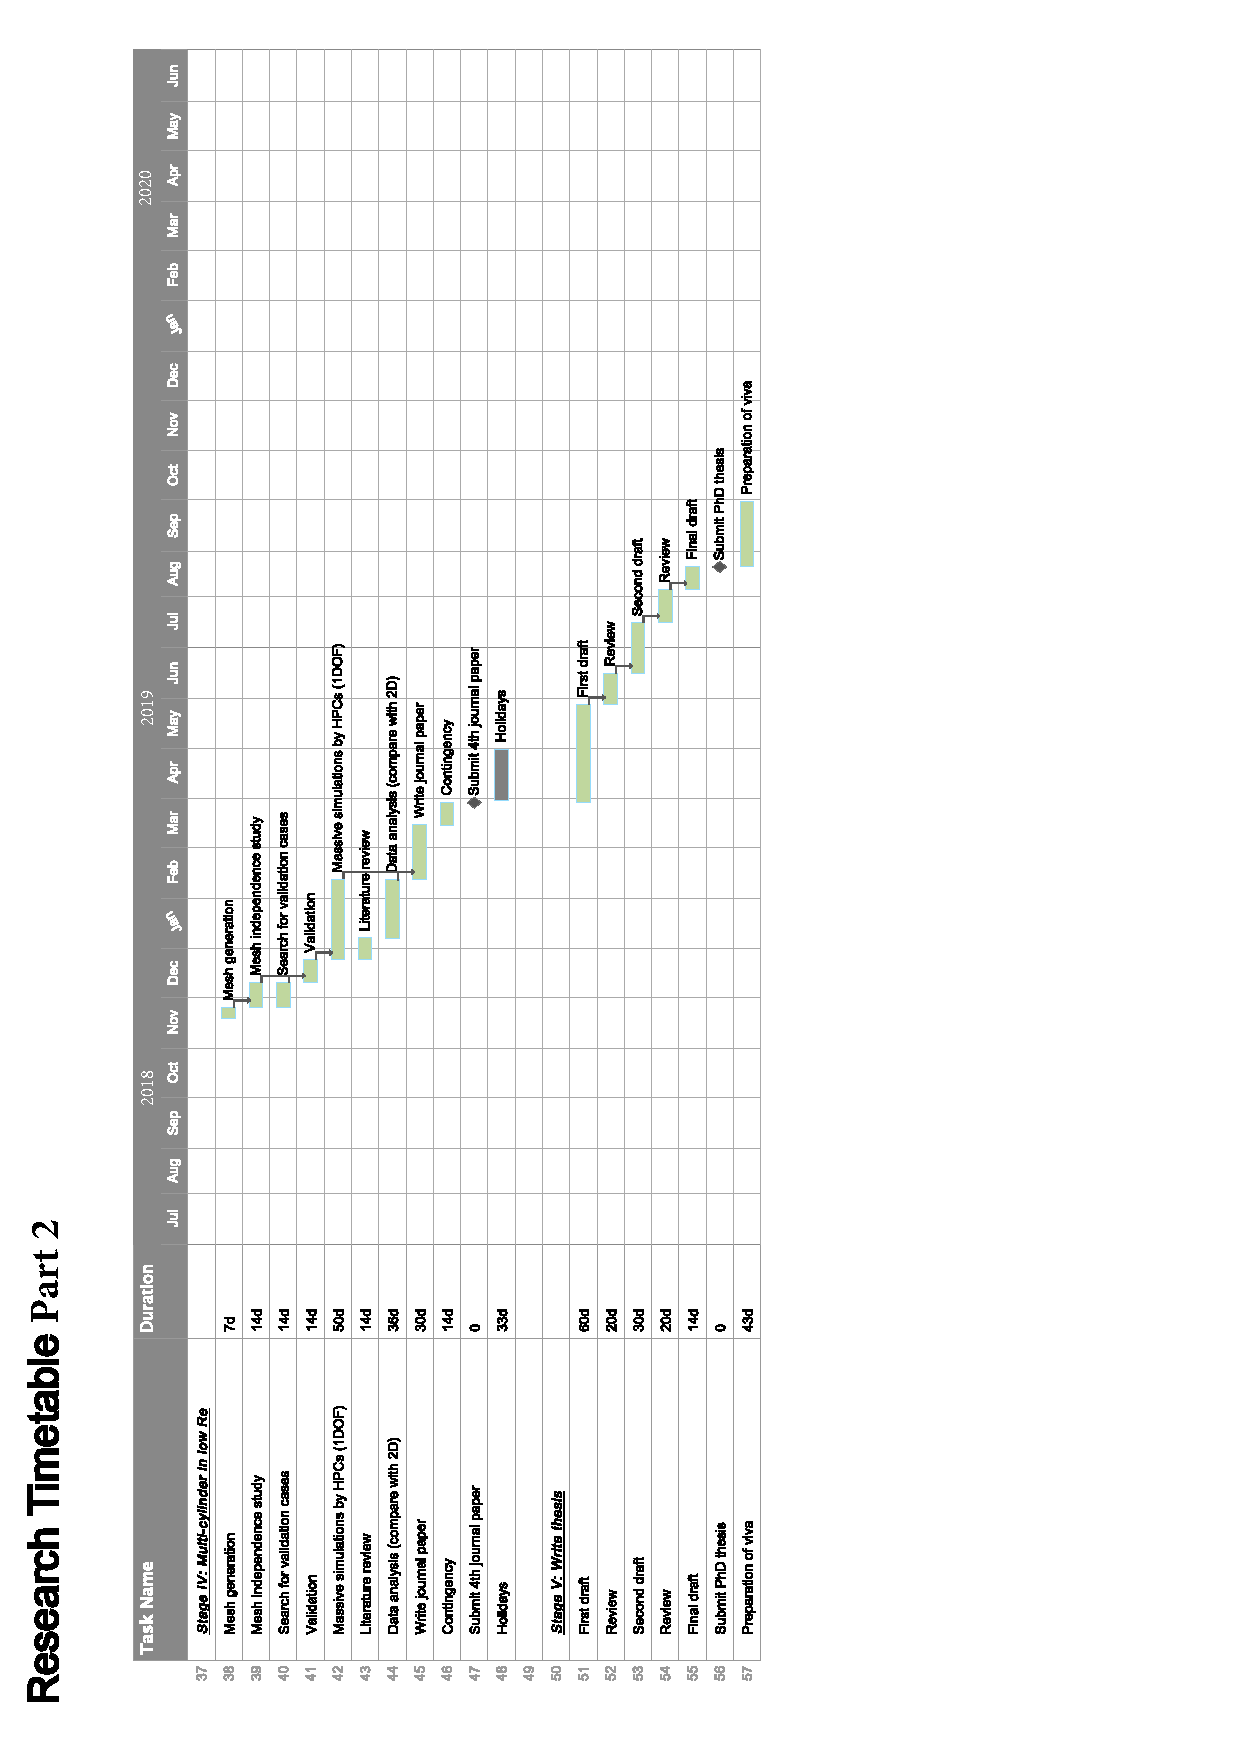
\includepdf[pages={1}]{Figs/Research Timetable (2)}


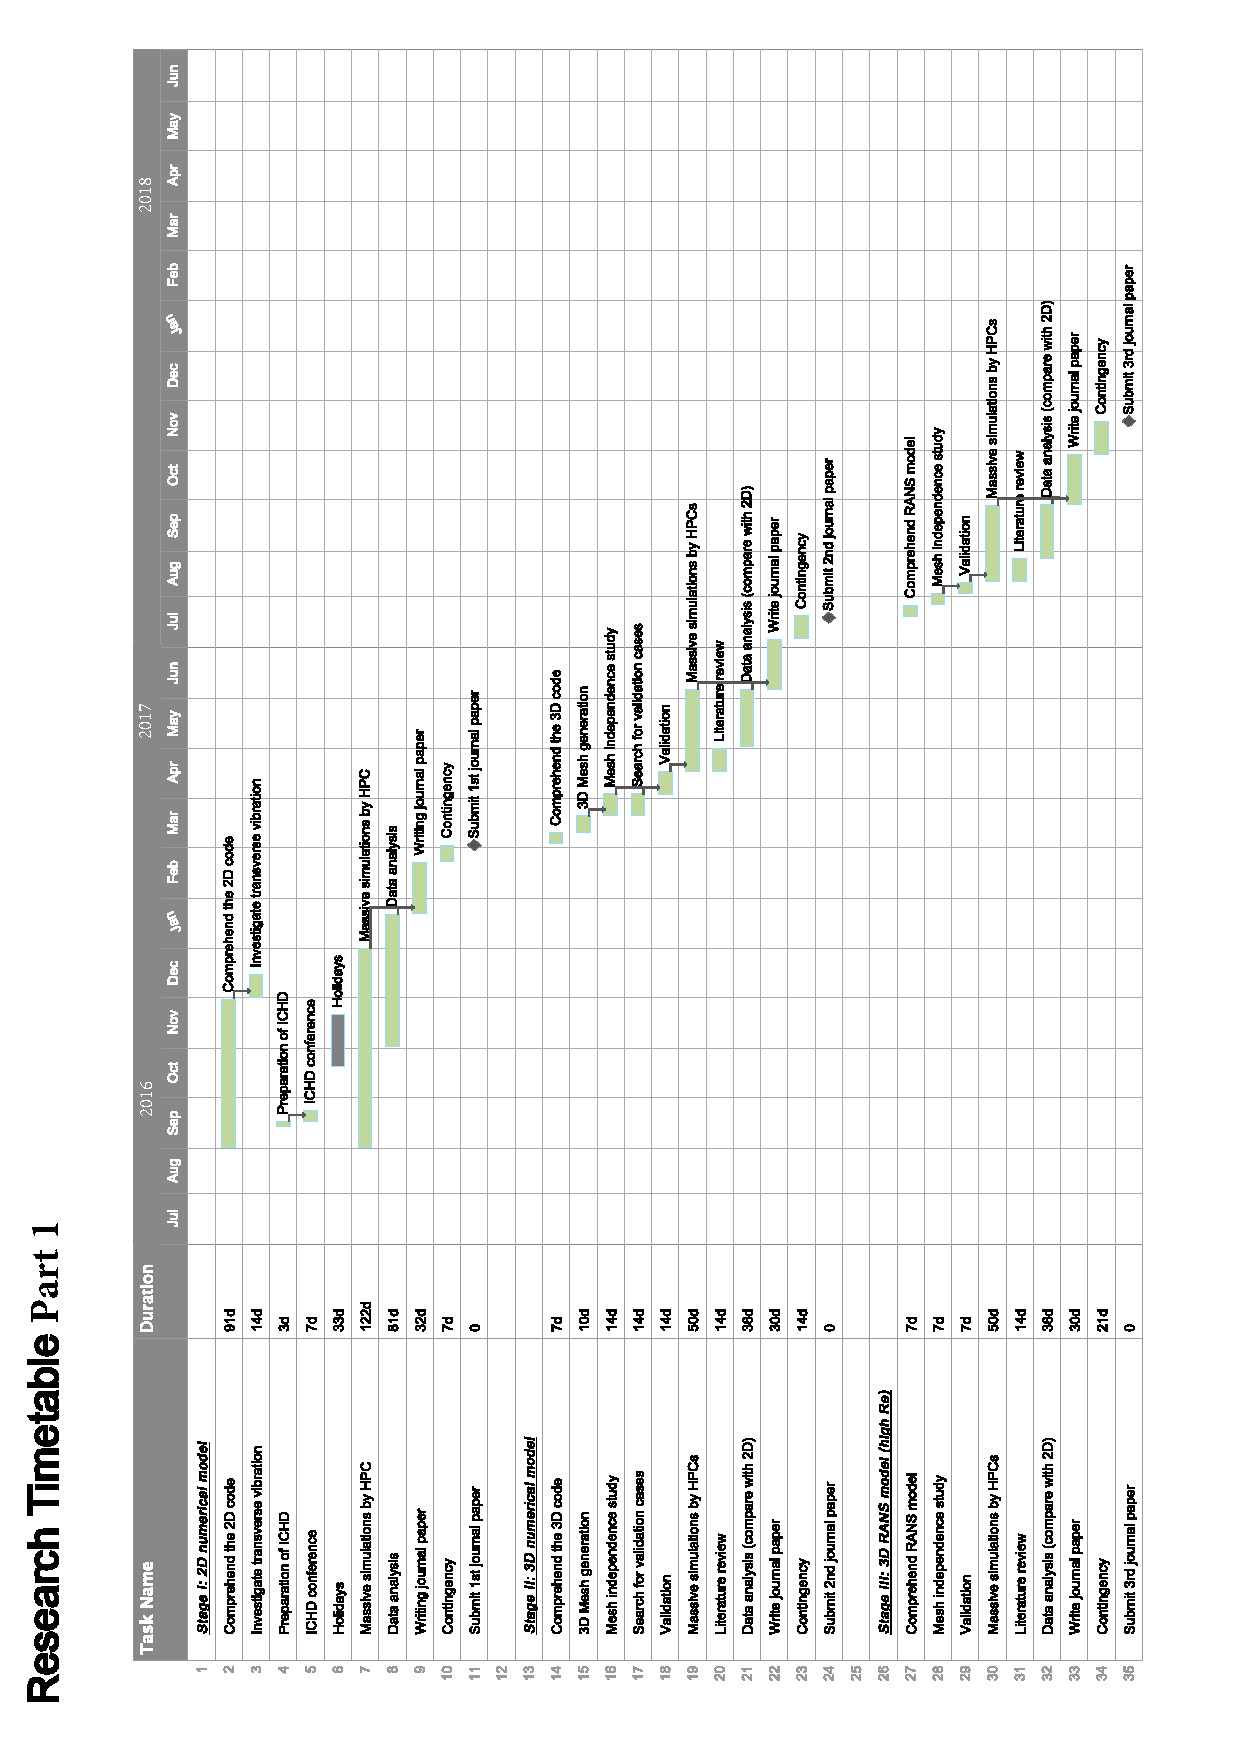
\includepdf{Figs/Research Timetable (1)}
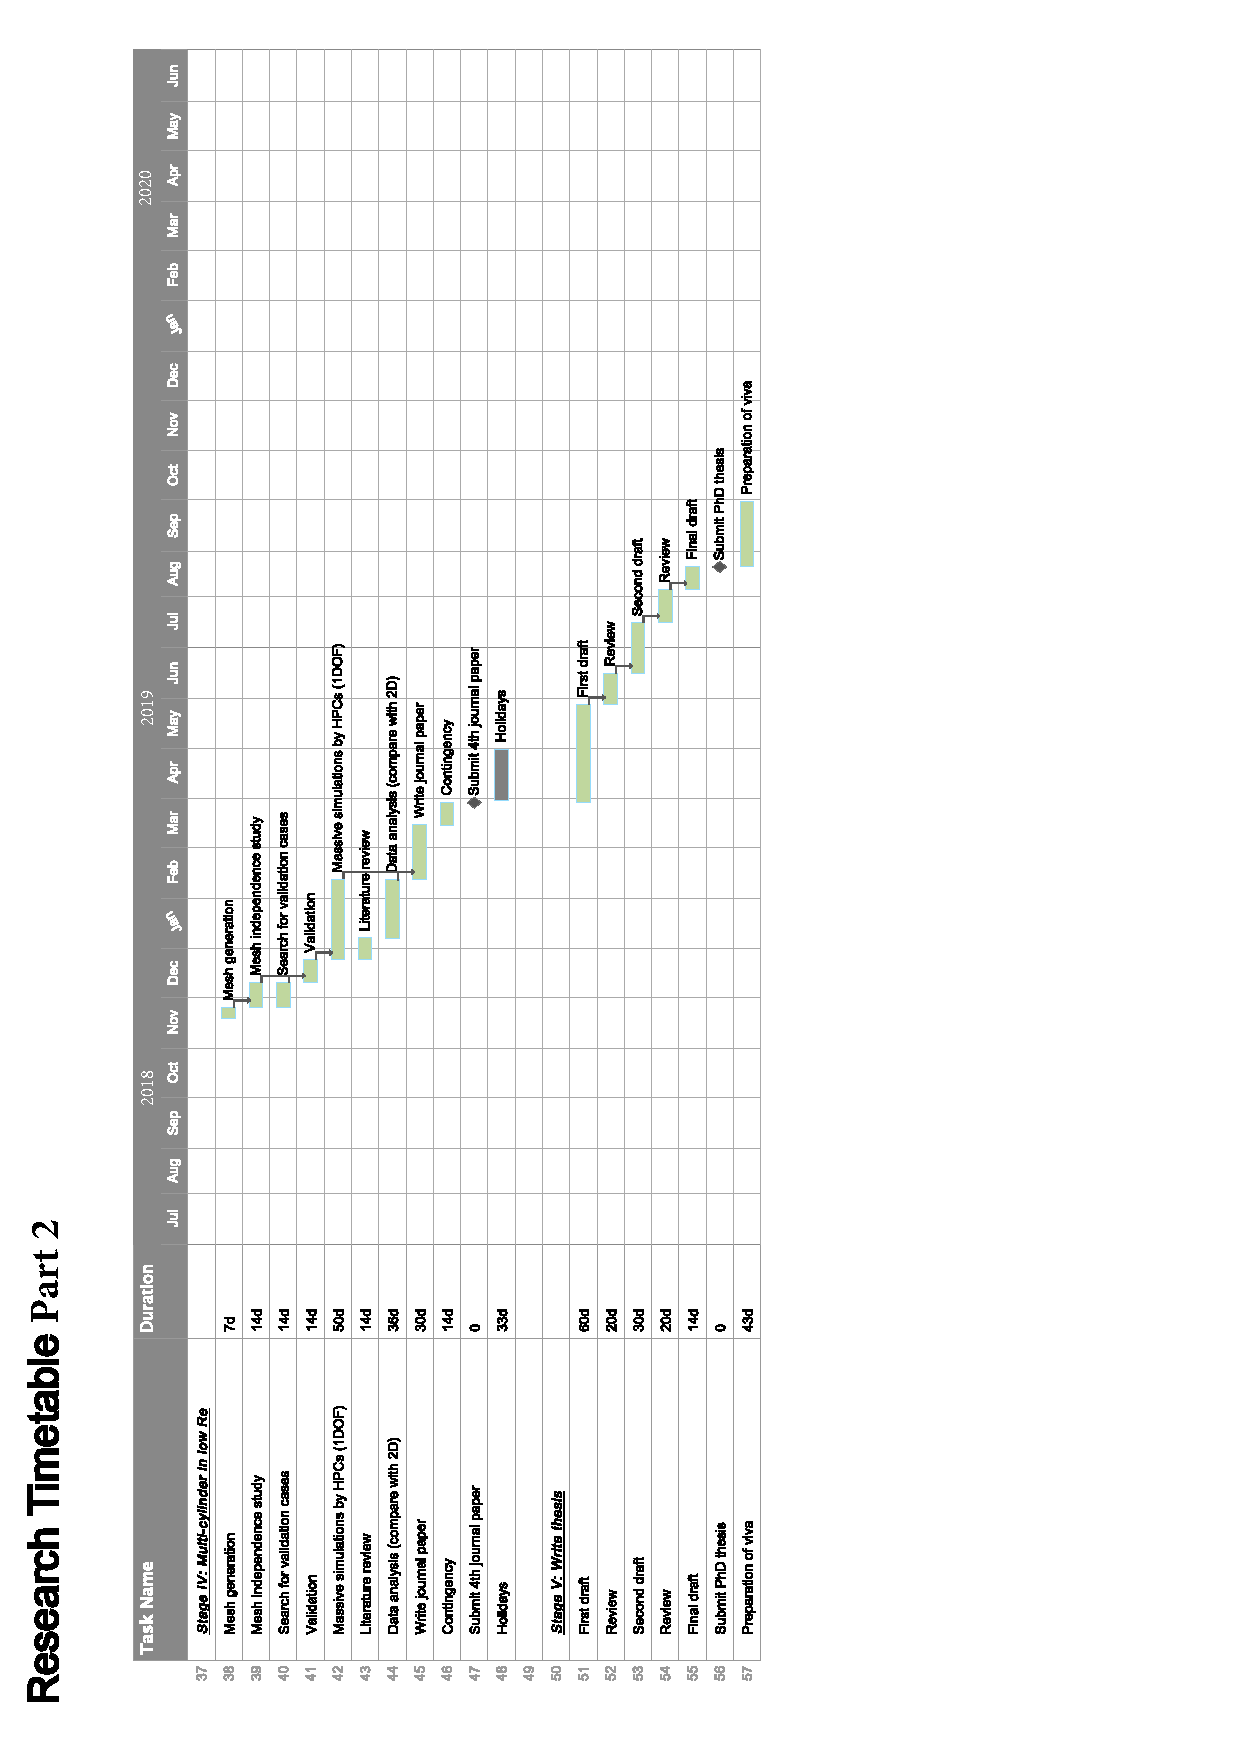
\includepdf{Figs/Research Timetable (2)}



%[14] Anagnostopoulos, P., and Iliadis, G., 1998, ?Numerical Study of the Flow Pat- tern and the In-Line Response of a Flexible Cylinder in an Oscillating Stream,? J. Fluids Struct., 12(3), pp. 225?258.
%[15] Mittal, S., and Kumar, V., 1999, ?Finite Element Study of Vortex-Induced Cross-Flow and In-Line Oscillations of a Circular Cylinder at Low Reynolds Numbers,? Int. J. Numer. Methods Fluids, 31(7), pp. 1087?1120.
%[16] Mittal, S., and Kumar, V., 2001, ?Flow-Induced Oscillations of Two Cylinders in Tandem and Staggered Arrangements,? J. Fluids Struct., 15(5), pp. 717?736.
%[17] Mittal, S., and Kumar, V., 2004, ?Vortex Induced Vibrations of a Pair of Cylinders at Reynolds Number 1000,? Int. J. Comput. Fluid Dyn., 18(7), pp. 601?614.
%[18] Jester, W., and Kallinderis, Y., 2004, ?Numerical Study of Incompressible Flow About Transversely Oscillating Cylinder Pairs,? ASME J. Offshore Mech. Arct. Eng., 126(4), pp. 310?317.
%[19] Zhao, M., 2013, ?Flow Induced Vibration of Two Rigidly Coupled Circular Cylinders in Tandem and Side-by- Side Arrangements at a Low Reynolds Num- ber of 150,? Phys. Fluids, 25(12), p. 123601.
